\documentclass[conference]{IEEEtran}

\usepackage[T1]{fontenc}
\usepackage[utf8]{inputenc}
\usepackage{amsmath}
\usepackage{array}
\usepackage{booktabs}
\usepackage{tabularx}
\usepackage{multirow}
\usepackage{xcolor}
\usepackage{graphicx}
\usepackage{tikz}
\usetikzlibrary{arrows.meta,positioning,fit,backgrounds,shapes.geometric,shapes.symbols}
\usepackage[hyphens]{url}
\usepackage[hidelinks]{hyperref}
\usepackage{minted}
\usepackage{balance}

\definecolor{zyalblue}{RGB}{37, 99, 168}
\definecolor{zyalgold}{RGB}{159, 119, 35}
\definecolor{zyalred}{RGB}{155, 54, 54}
\definecolor{zyalgreen}{RGB}{55, 130, 83}

\setminted{
  fontsize=\scriptsize,
  breaklines=true,
  breakanywhere=true,
  autogobble=true,
  frame=lines,
  framesep=1.5mm,
  tabsize=2
}

\newcommand{\ZYAL}{ZYAL}
\newcommand{\status}[1]{\textsf{\footnotesize #1}}
\newcommand{\shipped}{\status{shipped}}
\newcommand{\partialstatus}{\status{partial}}
\newcommand{\preview}{\status{preview}}

\begin{document}

\title{\ZYAL: A Host-Enforced Operating Contract for Autonomous Software Engineering Agents}

\author{\IEEEauthorblockN{Jekko Contributors}
\IEEEauthorblockA{Jankurai / Jekko Workspace\\
May 2026 Artifact Draft}}

\maketitle

\begin{abstract}
Autonomous software engineering agents now edit repositories, run tests, open pull requests, browse documentation, and coordinate with tools for many minutes or hours. The hard systems problem is no longer only whether a model can produce code; it is whether an operator can let an untrusted model act without surrendering stop conditions, budget control, safety policy, evidence discipline, and auditability. We present \ZYAL{} (Zero-Trust YAML Agent Language), a strict declarative runbook for governing long-running coding-agent daemons in the Jekko reference implementation. \ZYAL{} is not an agent SDK, prompt framework, or benchmark harness. It is a typed contract between a human operator and a host runtime: the model reasons, but the host parses, arms, persists, checks, checkpoints, routes, and stops. The current implementation includes a strict TypeScript schema and parser, SQLite-backed daemon state, HTTP preview/start APIs, a TUI run card, checkpoint and stop-check execution, task/incubator ledgers, and unit-tested helper modules for workflow, memory, evidence, approvals, security, sandboxing, observability, and guardrails. Higher-risk blocks such as hash/nonce arming, capability leases, anti-vibe quality gates, nested budgets, rollback, done definitions, and taint flow are intentionally treated as strict parser/preview contracts until every tool and promotion path is wired. This paper describes the design, implementation boundary, related systems, and artifact evidence for \ZYAL{} as a host-owned control plane for autonomous software engineering.
\end{abstract}

\begin{IEEEkeywords}
autonomous software engineering, AI agents, policy-as-code, agent safety, human-in-the-loop, YAML, zero trust, software agents
\end{IEEEkeywords}

\section{Introduction}

AI coding agents are moving from short pair-programming interactions toward autonomous engineering workflows: multi-file edits, shell execution, repository search, test repair, pull-request production, and long-running background work. Surveys of agentic programming identify planning, memory, tool integration, execution monitoring, safety, and human collaboration as central open problems rather than auxiliary features \cite{agenticProgrammingSurvey2025}. Empirical studies of agent-authored pull requests show that failed agentic PRs often involve larger changes, more files, CI failures, missing reviewer engagement, duplicate work, unwanted features, and agent-user misalignment \cite{failedAgenticPRs2026}. Security guidance likewise treats tool misuse, prompt injection, context hijacking, and insufficient human oversight as agentic threat classes \cite{owaspAgentic2026}.

These observations point to a structural gap. A prompt can tell an agent to be careful, run tests, respect secrets, and ask before dangerous actions. However, prompts are advisory text inside the same reasoning context that also contains untrusted repository files, tool output, web pages, and model-generated suggestions. For the safety properties that matter in autonomous software engineering, self-instruction is not enough. The process that decides when to start, which tools are exposed, how long work may run, what evidence is required, whether a patch can be promoted, and when the loop must stop should be outside the model.

\ZYAL{} is Jekko's answer to that gap. It is a strict YAML language wrapped in sentinels and interpreted by the host. A \ZYAL{} script declares the job, loop, stop checks, context rotation, checkpoint policy, tasks, incubator passes, permissions, MCP profiles, guardrails, workflows, memory stores, evidence bundles, approvals, sandbox and security settings, observability, and preview contracts for advanced governance blocks. The key design choice is not YAML itself; it is ownership. The host runtime owns continuation and enforcement. The language model is an executor whose output is evidence to inspect, not authority to trust.

The main contributions are:

\begin{itemize}
  \item A declarative operating contract for long-running software-engineering agents, with more than fifty recognized top-level keys organized into core, safety, evidence, security, power, fleet, taint, and control-plane-preview layers.
  \item A zero-trust arming and execution model that separates trusted host control from untrusted model output.
  \item A durable daemon architecture with SQLite state for runs, iterations, events, tasks, passes, memories, workers, and artifacts.
  \item A hard-task incubator that routes risky or stalled work through bounded scout, idea, critic, prototype, promotion, and compression passes.
  \item A proof-oriented artifact package: local claim audit, source register, framework matrix, diagrams, examples, build receipt, and reproducible PDF build.
\end{itemize}

This paper is careful about implementation status. Core parsing, preview, simple arming, daemon loop control, stop checks, checkpoint gating, state persistence, HTTP surfaces, TUI preview, task routing, and incubator machinery are shipped. Some helper modules are implemented and unit-tested but only partially integrated into the daemon loop. Several high-risk blocks are parser/preview contracts and must not be described as fully enforced.

Table~\ref{tab:failures} states the failure modes that motivated the contract. The table is also a useful reading guide: each row maps a social or empirical pain point to a host-owned mechanism rather than a stronger prompt.

\begin{table*}[t]
\centering
\caption{Agentic coding failure modes and \ZYAL{} countermeasures.}
\label{tab:failures}
\footnotesize
\begin{tabularx}{\textwidth}{p{28mm}p{42mm}p{44mm}X}
\toprule
Failure mode & Typical cause & \ZYAL{} countermeasure & Current status \\
\midrule
Unauthorized start & A model, tool, web page, or pasted block induces execution & Sentinels, explicit arm line, preview-before-start, future hash/nonce arming & Simple arm shipped; hash/nonce/origin preview \\
\midrule
Runaway loop & No host-owned stop check, error breaker, or budget & Loop policy, circuit breaker, stop checks, retry policy, budget contracts & Loop/stop/breaker shipped; nested budgets preview \\
\midrule
Unsafe shell/tool use & Coarse allow/deny or user fatigue with prompts & Permissions, MCP profiles, command floor, capability leases, sandbox and security blocks & Permissions/MCP partial; leases/sandbox/security not fully wired \\
\midrule
Vibe-coded regression & Tests deleted, assertions weakened, type errors hidden, fake fallbacks added & Quality anti-vibe gates, diff budgets, evidence before promotion & Parser/preview contract \\
\midrule
False completion & Model claims done without proof & Host-evaluated stop checks, evidence bundles, workflow gates, approvals, done definitions & Stop/checkpoint shipped; evidence/workflow partial; done preview \\
\midrule
Repeated dead ends & Context eviction loses failed hypotheses & Incubator passes, task memory, negative findings, promotion/exhaustion ledgers & Core incubator shipped \\
\midrule
Unreviewable output & Large diffs and missing audit trail & SQLite events, task/pass memory, artifact records, checkpoint SHAs, TUI/API inspection & Shipped for daemon and incubator paths \\
\bottomrule
\end{tabularx}
\end{table*}

\section{Background and Related Work}

Most agent systems expose one of four surfaces: a programming SDK, an orchestration graph, a coding-agent runtime, or a protocol/configuration substrate. \ZYAL{} borrows from all four, but its narrow goal is different: it specifies what the host must enforce before, during, and after autonomous repository work.

Graph and SDK systems such as LangGraph, OpenAI Agents SDK, Microsoft Agent Framework, CrewAI, LlamaIndex, PydanticAI, Haystack, Semantic Kernel, Google ADK, smolagents, Mastra, and VoltAgent provide useful agent abstractions, workflows, tool definitions, persistence, memory, telemetry, and human-in-the-loop hooks \cite{langgraphPersistence2026,openaiAgentsSdk2026,microsoftAgentFramework2026,crewaiDocs2026,llamaIndexAgents2026,pydanticAiAgents2026,haystackAgents2026,semanticKernelAgents2026,googleAdk2026,smolagents2026,mastra2026,voltagent2026}. Multi-agent research systems such as AutoGen, MetaGPT, and CAMEL explore conversable agents, software-company SOPs, and role-playing collaboration \cite{autogen2023,metagpt2023,camel2023}. Coding-agent runtimes such as OpenHands, SWE-agent, Aider, Claude Code, Codex CLI, Devin, Cursor, Windsurf, and Hermes Agent/OpenClaw expose repository editing, shell execution, sandboxes, checkpoints, codebase context, or PR workflows \cite{openhands2024,sweAgent2024,aiderDocs2026,claudeCodePermissions2026,codexCliHelp2026,devinDocs2026,cursorAgentDocs2026,windsurfCascade2026,hermesAgentRepo2026}. Finally, MCP, OpenAPI, OPA/Rego, GitHub Actions, Kubernetes, and Terraform show the value of protocol boundaries, machine-readable contracts, policy-as-code, YAML automation, and declarative desired state \cite{mcpDocs2026,openApiSpec2026,opaRego2026,githubActionsSyntax2026,kubernetesDeclarative2023,terraformIac2026}.

Table~\ref{tab:related} compresses the detailed matrix in \texttt{paper/research/framework-matrix.md}. The table is intentionally not a ranking. Mature frameworks are strong within their design centers. The \ZYAL{} distinction is that the contract is external to the model and evaluated by the host as an operating boundary.

\begin{table*}[t]
\centering
\caption{Related systems and the \ZYAL{} distinction. The full matrix includes scripting abstraction, strengths, limitations, safety boundary, memory/context story, observability, and human approval model for each named system.}
\label{tab:related}
\footnotesize
\begin{tabularx}{\textwidth}{p{27mm}p{39mm}X}
\toprule
Family & Examples & Contrast with \ZYAL{} \\
\midrule
Agent SDKs and graphs & LangChain, LangGraph, LlamaIndex, PydanticAI, Haystack, Semantic Kernel, Microsoft Agent Framework, OpenAI Agents SDK, Google ADK, smolagents, Mastra, VoltAgent & These systems provide agents, tools, workflows, memory, persistence, tracing, or deployment. \ZYAL{} specifies a host-owned run contract with explicit arming, stop checks, checkpoint policy, evidence, task routing, and preview limitations. \\
\midrule
Multi-agent research and role systems & AutoGen, CrewAI, MetaGPT, CAMEL, AutoGPT, BabyAGI & These systems organize agent collaboration through conversation, crews, roles, SOPs, or task queues. \ZYAL{} treats collaboration as subordinate to a typed host contract, bounded passes, finite budgets, durable ledgers, and promotion gates. \\
\midrule
Coding-agent runtimes & OpenHands, SWE-agent, Aider, Claude Code, Codex CLI, Devin, Cursor/Windsurf agents, Hermes Agent/OpenClaw & These systems expose practical software-engineering capabilities. \ZYAL{} is designed to govern such capabilities: what may run, when it must stop, what evidence is required, and which preview policies are not yet enforceable. \\
\midrule
Protocols and declarative precedents & MCP, function/tool schemas, OpenAPI, OPA/Rego, GitHub Actions, Kubernetes, Terraform & These systems motivate machine-readable contracts, policy decisions, and host reconciliation. \ZYAL{} applies that style to autonomous coding-agent sessions rather than APIs, infrastructure, or CI alone. \\
\bottomrule
\end{tabularx}
\end{table*}

\section{Language Design}

\subsection{Sentinel Format}

A \ZYAL{} block is structurally distinct from Markdown and code fences:

\begin{minted}{yaml}
<<<ZYAL v1:daemon id=my-script>>>
version: v1
intent: daemon
confirm: RUN_FOREVER
job:
  name: "Fix until green"
  objective: "Make the failing lane pass."
stop:
  all:
    - shell:
        command: "bun test"
        assert: { exit_code: 0 }
<<<END_ZYAL id=my-script>>>
ZYAL_ARM RUN_FOREVER id=my-script
\end{minted}

The parser accepts only blank lines or comments before the opening sentinel, rejects code fences, rejects duplicate blocks, requires matching open/close IDs, rejects arbitrary trailing content, and validates that the optional arm line matches the block ID. The start path requires the trailing arm sentinel; preview mode can parse without it.

\subsection{Block Layers}

The schema groups language blocks into evolutionary layers:

\begin{itemize}
  \item Core: \texttt{version}, \texttt{intent}, \texttt{confirm}, \texttt{id}, \texttt{job}, \texttt{loop}, \texttt{stop}, \texttt{context}, \texttt{checkpoint}, \texttt{tasks}, \texttt{incubator}, \texttt{agents}, \texttt{mcp}, \texttt{permissions}, \texttt{ui}.
  \item Safety: \texttt{on}, \texttt{fan\_out}, \texttt{guardrails}, \texttt{assertions}, \texttt{retry}, \texttt{hooks}, \texttt{constraints}.
  \item Evidence and governance: \texttt{workflow}, \texttt{memory}, \texttt{evidence}, \texttt{approvals}, \texttt{skills}, \texttt{sandbox}, \texttt{security}, \texttt{observability}.
  \item Power and preview: \texttt{arming}, \texttt{capabilities}, \texttt{quality}, \texttt{experiments}, \texttt{models}, \texttt{budgets}, \texttt{triggers}, \texttt{rollback}, \texttt{done}, \texttt{repo\_intelligence}, \texttt{fleet}, \texttt{taint}, and control-plane metadata such as \texttt{interop}, \texttt{runtime}, \texttt{evidence\_graph}, \texttt{trust}, \texttt{roles}, \texttt{channels}, \texttt{imports}, and \texttt{unsupported\_feature\_policy}.
\end{itemize}

The implementation source of truth is \texttt{packages/jekko/src/agent-script/schema.ts}, currently 2,078 lines and 85,727 bytes, and \texttt{parser.ts}, currently 1,803 lines and 75,355 bytes. Parser tests cover bundled examples and all ten canonical documentation examples under \texttt{docs/ZYAL/examples/}.

\subsection{Implementation Coverage}

Table~\ref{tab:coverage} summarizes the claim boundary used throughout the paper. The detailed evidence is maintained in \texttt{paper/research/claim-audit.md}. The point of the table is not to minimize unfinished work; it is to prevent a preview contract from being accidentally marketed as a completed security mechanism.

\begin{table*}[t]
\centering
\caption{\ZYAL{} block-family implementation status in the current reference implementation.}
\label{tab:coverage}
\footnotesize
\begin{tabularx}{\textwidth}{p{29mm}p{16mm}X}
\toprule
Block family & Status & Evidence and boundary \\
\midrule
Sentinels, strict keys, schema decode, semantic parser checks & \shipped & \texttt{parser.ts}, \texttt{schema.ts}, and parser tests reject malformed blocks, duplicate blocks, code fences, unknown keys, invalid incubator budgets, invalid fleet caps, and invalid taint references. \\
\midrule
Simple arming and preview & \shipped & The daemon start path requires a trailing arm sentinel. Preview parses without starting and powers the TUI run card. \\
\midrule
Daemon loop, stop checks, checkpoint gating, context rotation & \shipped & \texttt{daemon.ts}, \texttt{daemon-checks.ts}, and \texttt{daemon-checkpoint.ts} own iteration, shell/git stop checks, verification, commit behavior, and context fork points. \\
\midrule
SQLite run/task/pass/memory/artifact ledgers & \shipped & \texttt{daemon.sql.ts} and \texttt{daemon-store.ts} persist runs, iterations, events, tasks, passes, task memories, workers, and artifacts. \\
\midrule
Incubator routing and promotion & \shipped & \texttt{daemon-incubator.ts}, \texttt{daemon-task-router.ts}, and \texttt{daemon-task-promote.ts} implement bounded passes, readiness routing, worktree prototypes, and promotion/exhaustion gates. \\
\midrule
\texttt{on}, hooks, retry, constraints, guardrail helpers & \partialstatus & Helpers and tests exist; the daemon loop uses on-handlers, hooks, retry for stop evaluation, and circuit breakers. Guardrail/constraint coverage is not yet universal across all tool paths. \\
\midrule
Workflow, memory, evidence, approvals, skills, sandbox, security, observability & \partialstatus & Unit-tested helper modules exist and preview summaries are available, but full daemon-loop enforcement is selective. \\
\midrule
Hash/nonce arming, capability leases, quality gates, nested budgets, triggers, rollback, done, repo intelligence, taint, control-plane metadata & \preview & Parser/preview contracts and examples exist. These blocks must be displayed as future enforcement requirements until all runtime boundaries call them. \\
\bottomrule
\end{tabularx}
\end{table*}

\subsection{Preview as a First-Class Mode}

Preview mode is not a convenience feature; it is part of the safety model. It lets the host parse, validate, summarize, hash, and display a run card without execution. The TUI run card reports objective, armed/draft status, loop policy, stop checks, checkpoint checks, worker count, fleet summary, incubator summary, arming preview, capability rules, budgets, taint labels, unsupported-feature policy, and risks. The run card also states that arming hash/nonce/origin and taint flow are preview-only until end-to-end runtime enforcement exists.

\subsection{Host Invariants}

The language is organized around invariants that the model is not allowed to satisfy by assertion. A model may say that tests passed, a command is safe, a change is small, or a task is ready to promote, but the daemon must reduce those claims to host-observed facts before changing run state. This is the practical distinction between a runbook and an operating contract. The runbook tells an assistant what to do; the operating contract tells the host which state transitions are legal.

Table~\ref{tab:invariants} lists the invariants used while auditing the current implementation. Each invariant has a shipped, partial, or preview boundary because the useful unit of safety is not the schema field alone. It is the combination of parse-time validation, preview visibility, execution-time enforcement, durable evidence, and user-facing status. For example, a capability lease that parses correctly but is not consulted by every command path is a design requirement, not yet a security boundary. Conversely, a stop check is stronger because the daemon actually runs it and records the result before completion.

\begin{table*}[t]
\centering
\caption{Host invariants used to separate enforceable behavior from preview contracts.}
\label{tab:invariants}
\footnotesize
\begin{tabularx}{\textwidth}{p{30mm}p{38mm}p{44mm}X}
\toprule
Invariant & Host-owned decision & Implementation evidence & Boundary \\
\midrule
Start authority & A daemon run starts only from a syntactically valid block plus an explicit arming line accepted by the start path. & Parser sentinels, ID matching, trailing-arm validation, preview/start API split. & Simple arming shipped; hash, nonce, origin, and single-use arming are preview. \\
\midrule
Continuation authority & The host, not the model, decides whether another iteration is legal. & Loop counters, circuit breaker state, stop checks, checkpoint results, pause/abort/resume transitions, event records. & Shipped for daemon loop and stop/checkpoint gates. \\
\midrule
Evidence authority & Completion and promotion require host-visible artifacts rather than assistant prose. & Shell check receipts, git-clean checks, checkpoint SHAs, task pass receipts, artifact rows, evidence bundle helpers. & Shipped for stop/checkpoint and incubator receipts; evidence bundles are partial. \\
\midrule
Privilege authority & Tools, shell commands, MCP profiles, paths, and publication actions must pass host policy before execution or exposure. & Permission profiles, MCP preview summaries, push-as-approval pause, sandbox/security/capability schemas. & Partial today; capability leases and command floors are preview until consulted on every tool path. \\
\midrule
Memory authority & Repeated failures and promoted decisions should become durable, inspectable state rather than hidden prompt residue. & Task memory table, incubator negative memory, memory helper provenance/redaction rules, generated mirror receipts. & Incubator memory shipped; generalized memory kernel is partial/preview depending on path. \\
\midrule
Unsupported-feature authority & A script that asks for host guarantees the runtime cannot provide should fail closed or visibly degrade, never silently pretend. & Strict parser keys, preview summary warnings, unsupported-feature policy schema, claim audit. & Parser and preview shipped; cross-host negotiation remains preview. \\
\bottomrule
\end{tabularx}
\end{table*}

\section{Threat Model and Safety Model}

\subsection{Model as Untrusted Executor}

\ZYAL{} assumes the model is useful but not trusted. It can hallucinate, omit evidence, overstate readiness, follow malicious instructions embedded in tool output, ask for unnecessary privileges, or generate unsafe commands. External content, MCP resources, issue comments, repository files, and assistant output are not trusted origins for arming or privilege escalation.

The trusted computing base is the local host process: parser, schema decoder, daemon state machine, permission/tool layer, durable store, and user-facing control surfaces. \ZYAL{} does not defend against a compromised host binary, malicious kernel, provider-side logging, or operating-system account compromise. Its narrower claim is testable: model output should not bypass host checks that are actually wired into the runtime.

\subsection{Host Control Loop}

Fig.~\ref{fig:host-loop} shows the control loop. The host accepts a typed script, requires explicit arming for start, persists the run, prompts the model for one iteration, records token/cost/result data, checkpoints verified changes, evaluates stop checks, routes hard tasks through the incubator, appends continuation prompts, rotates context when configured, and sleeps. The model never owns the loop.

\begin{figure*}[t]
\centering
\resizebox{\textwidth}{!}{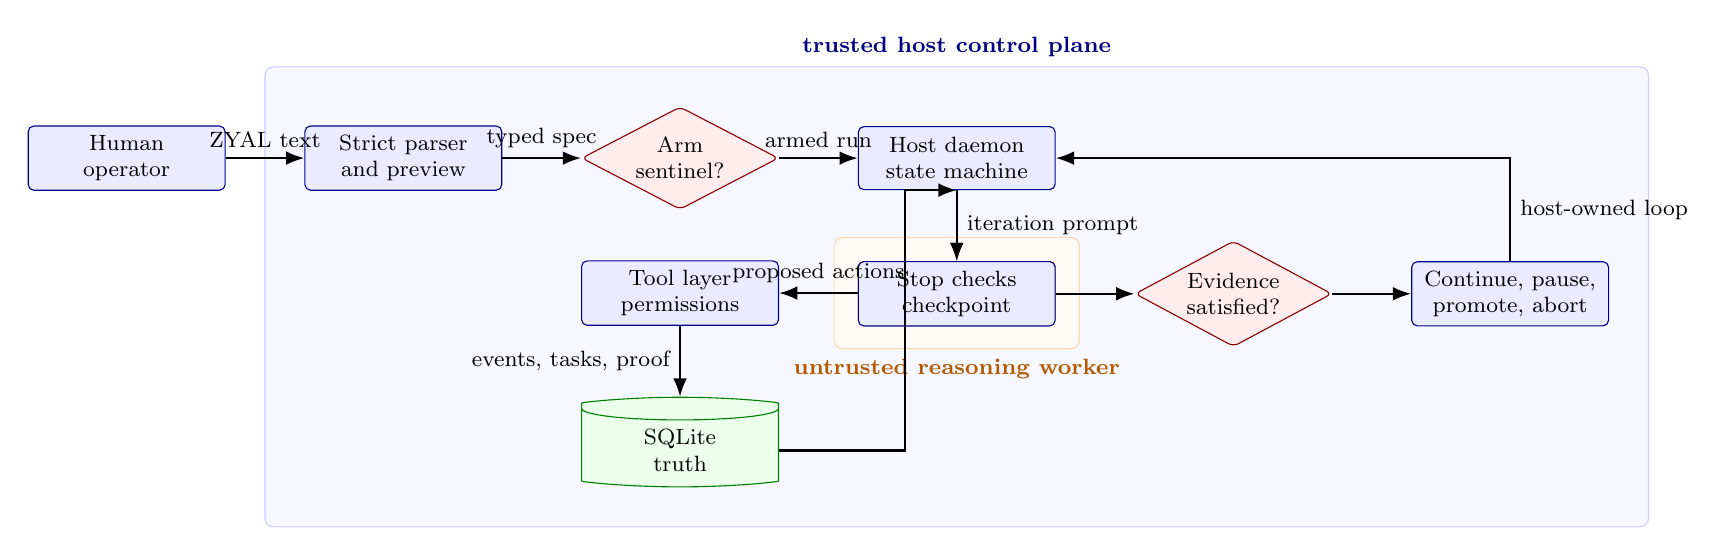
\begin{tikzpicture}[
  font=\footnotesize,
  >=Latex,
  node distance=9mm and 10mm,
  box/.style={draw, rounded corners=2pt, align=center, minimum width=25mm, minimum height=8mm, fill=white},
  host/.style={box, fill=blue!8, draw=blue!55!black},
  model/.style={box, fill=orange!10, draw=orange!70!black},
  store/.style={box, cylinder, shape border rotate=90, aspect=0.25, minimum height=10mm, fill=green!8, draw=green!50!black},
  gate/.style={box, diamond, aspect=1.7, fill=red!7, draw=red!55!black, inner sep=1pt},
  edge/.style={->, thick}
]
\node[host] (human) {Human\\operator};
\node[host, right=of human] (parser) {Strict parser\\and preview};
\node[gate, right=of parser] (arm) {Arm\\sentinel?};
\node[host, right=of arm] (runtime) {Host daemon\\state machine};
\node[model, below=of runtime] (model) {LLM executor\\untrusted};
\node[host, left=of model] (tools) {Tool layer\\permissions};
\node[store, below=of tools] (sqlite) {SQLite\\truth};
\node[host, below=of runtime] (checks) {Stop checks\\checkpoint};
\node[gate, right=of checks] (evidence) {Evidence\\satisfied?};
\node[host, right=of evidence] (next) {Continue, pause,\\promote, abort};

\draw[edge] (human) -- node[above] {ZYAL text} (parser);
\draw[edge] (parser) -- node[above] {typed spec} (arm);
\draw[edge] (arm) -- node[above] {armed run} (runtime);
\draw[edge] (runtime) -- node[right] {iteration prompt} (model);
\draw[edge] (model) -- node[above] {proposed actions} (tools);
\draw[edge] (tools) -- node[left] {events, tasks, proof} (sqlite);
\draw[edge] (runtime) -- (checks);
\draw[edge] (checks) -- (evidence);
\draw[edge] (evidence) -- (next);
\draw[edge] (next.north) |- node[pos=0.25,right] {host-owned loop} (runtime.east);
\draw[edge] (sqlite.east) -- ++(16mm,0) |- (runtime.south);

\begin{scope}[on background layer]
\node[draw=blue!20, fill=blue!3, rounded corners=3pt, fit=(parser)(arm)(runtime)(tools)(checks)(evidence)(next)(sqlite), inner sep=5mm,
  label={[font=\footnotesize\bfseries, text=blue!50!black]above:trusted host control plane}] {};
\node[draw=orange!30, fill=orange!4, rounded corners=3pt, fit=(model), inner sep=3mm,
  label={[font=\footnotesize\bfseries, text=orange!70!black]below:untrusted reasoning worker}] {};
\end{scope}
\end{tikzpicture}
}
\caption{Host-owned \ZYAL{} control loop. The model proposes work; the host controls arming, iteration, evidence, checkpointing, persistence, and termination.}
\label{fig:host-loop}
\end{figure*}

\subsection{Arming and Capability Leases}

The shipped start path enforces the simple sentinel \texttt{ZYAL\_ARM RUN\_FOREVER id=<id>}. Hash-bound, nonce-bound, single-use, and accepted-origin arming policies are parsed and summarized but are preview-only until the start API carries host-issued tokens. This distinction is essential: a paper that claims full nonce enforcement today would be wrong.

The \texttt{capabilities} block describes leases over tools, paths, commands, MCP profiles, and expiration windows. It also defines a command floor that no allow rule should override. The schema and preview support are present, but full enforcement requires every tool path to consult the lease evaluator before execution. For now, capability leases are a design contract and parser/preview artifact, not a completed security boundary.

\subsection{Taint Flow}

The v2.3 \texttt{taint} block labels inbound bytes by origin and rank and can forbid tainted sources from triggering privileged actions such as \texttt{arm}, \texttt{approve}, \texttt{grant\_capability}, \texttt{exec\_shell}, or \texttt{expose\_secret}. The parser validates labels, references, action lists, and injection-pattern regexes. Execution-time taint propagation is not yet wired into the daemon loop, so it is labelled preview. Fig.~\ref{fig:taint} shows the intended flow.

\begin{figure*}[t]
\centering
\resizebox{\textwidth}{!}{\begin{tikzpicture}[
  font=\footnotesize,
  >=Latex,
  node distance=8mm and 8mm,
  box/.style={draw, rounded corners=2pt, align=center, minimum width=23mm, minimum height=8mm, fill=white},
  taint/.style={box, fill=red!8, draw=red!55!black},
  cap/.style={box, fill=blue!8, draw=blue!55!black},
  gate/.style={box, diamond, aspect=1.7, fill=yellow!12, draw=yellow!55!black, inner sep=1pt},
  sink/.style={box, fill=green!8, draw=green!50!black},
  edge/.style={->, thick}
]
\node[box] (source) {Source origin\\user, repo, tool, web, MCP};
\node[taint, right=of source] (label) {Taint label\\rank + provenance};
\node[gate, right=of label] (action) {Privileged\\action?};
\node[cap, above right=of action] (lease) {Capability lease\\tool, path, time};
\node[gate, right=of action] (floor) {Command\\floor};
\node[gate, right=of floor] (approval) {Human or\\signed sanitizer};
\node[sink, right=of approval] (exec) {Execution\\and event log};
\node[taint, below=of action] (deny) {Fail closed\\pause or reject};

\draw[edge] (source) -- (label);
\draw[edge] (label) -- (action);
\draw[edge] (action) -- node[above left] {needs grant} (lease);
\draw[edge] (lease) -| (floor);
\draw[edge] (action) -- node[above] {low risk} (floor);
\draw[edge] (floor) -- node[above] {not blocked} (approval);
\draw[edge] (approval) -- node[above] {approved} (exec);
\draw[edge] (action) -- node[right] {tainted high-risk} (deny);
\draw[edge] (floor) |- node[pos=0.25,right] {always block} (deny);
\draw[edge] (approval) |- node[pos=0.25,right] {missing approval} (deny);
\end{tikzpicture}
}
\caption{Trust, capability, and taint flow. High-risk actions require a compatible lease, must pass the command floor, and may require human approval or signed sanitization.}
\label{fig:taint}
\end{figure*}

\section{Runtime Architecture}

\subsection{Daemon Loop}

The daemon service exposes preview, start, list, get, events, task inspection, task pass history, task memory, task actions, incubator state, pause, resume, abort, compact, and rotate-session methods. The HTTP layer maps these to routes such as \texttt{/daemon/preview}, \texttt{/session/:sessionID/daemon/start}, \texttt{/daemon/:runID/events}, and \texttt{/daemon/:runID/tasks/:taskID/memory}. The route definitions and handlers are covered by \texttt{httpapi-daemon.test.ts}.

The loop itself is in \texttt{packages/jekko/src/session/daemon.ts}. It records each assistant iteration, tracks signal counters, evaluates \texttt{on} handlers, applies the circuit breaker, runs checkpoint verification, evaluates stop checks with retry policy, routes tasks through the incubator, appends a continuation prompt, optionally forks the session for hard context rotation, and sleeps. Status and phase transitions are published on the bus so the UI can display live state.

\subsection{SQLite Truth and Generated Mirrors}

The durable store uses eight daemon-specific SQLite tables:

\begin{table}[t]
\centering
\caption{Daemon SQLite tables in the reference implementation.}
\label{tab:tables}
\footnotesize
\begin{tabularx}{\columnwidth}{p{29mm}X}
\toprule
Table & Purpose \\
\midrule
\texttt{daemon\_run} & run metadata, active session, status, phase, spec hash \\
\texttt{daemon\_iteration} & per-iteration terminal reason, token usage, cost, checkpoint SHA \\
\texttt{daemon\_event} & append-only event stream \\
\texttt{daemon\_task} & task ledger, lane, risk/readiness/confidence, lease fields \\
\texttt{daemon\_task\_pass} & incubator pass lifecycle, worktree, artifacts, result scores \\
\texttt{daemon\_task\_memory} & findings, objections, decisions, receipts, negative memory \\
\texttt{daemon\_worker} & worker leases, sessions, branches, heartbeat status \\
\texttt{daemon\_artifact} & evidence, diffs, bundles, rollback artifacts \\
\bottomrule
\end{tabularx}
\end{table}

The database is the authority. Human-readable files under generated daemon mirrors are inspection artifacts and should be treated as generated output.

\subsection{Checkpoint and Stop Evaluation}

Stop conditions support shell checks and git-clean checks. Shell assertions can check exit code, stdout substrings, stdout regexes, and JSON paths. Checkpoints run configured verification commands before staging and committing. If the tree is clean and \texttt{noop\_if\_clean} is true, checkpointing can no-op. If \texttt{git.push} is \texttt{ask}, the checkpoint path returns a pause reason instead of pushing. This models a common safety rule: a host may create verified local state, but externally visible publication needs a separate decision.

\section{Incubation, Evidence, and Memory}

Hard repository tasks often fail because a single linear attempt overfits to the first plausible diagnosis. \ZYAL{} provides an incubator for tasks that are risky, repeated, or stalled. The parser rejects unbounded incubator budgets, non-positive counts, unknown pass types, unknown context modes, \texttt{main\_worktree} writes before promotion, prototype passes without scratch/worktree isolation, and idea fanout that exceeds configured limits. Fleet caps also constrain agents, fan-out, experiments, and incubator concurrency.

At runtime, the incubator routes candidate tasks by risk, readiness, no-progress count, repeated attempts, and path patterns. It stores task memories, starts typed passes, creates isolated worktrees for prototype passes, records pass receipts, evaluates promotion requirements, and either promotes, parks, blocks, archives, or continues. Fig.~\ref{fig:incubator} summarizes the tournament pattern.

\begin{figure*}[t]
\centering
\resizebox{\textwidth}{!}{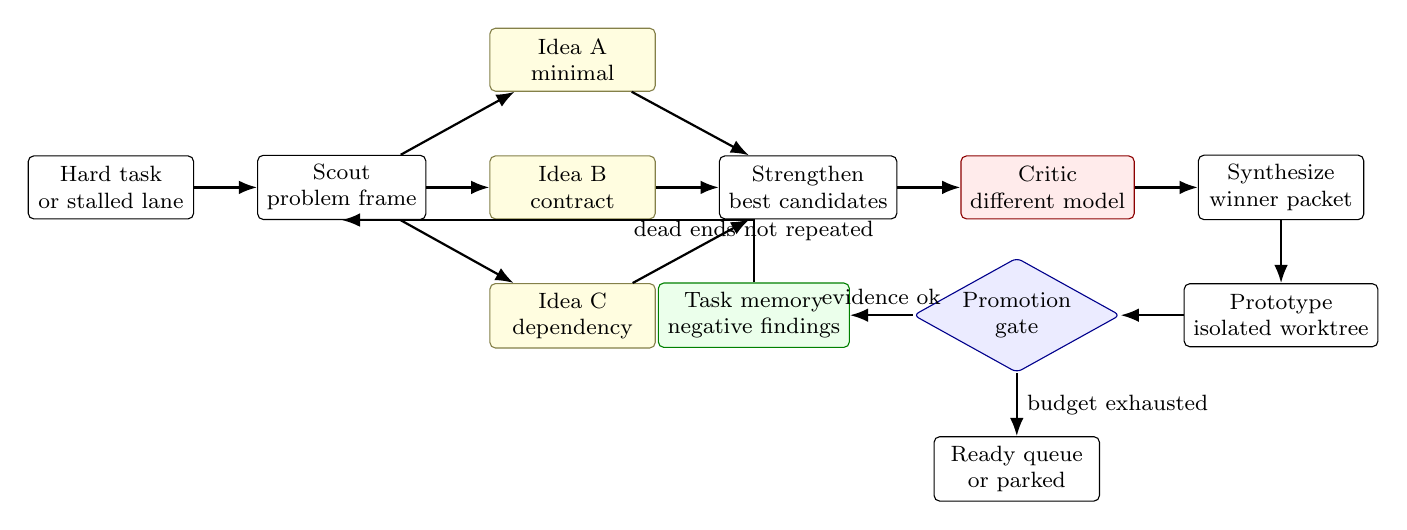
\begin{tikzpicture}[
  font=\footnotesize,
  >=Latex,
  node distance=8mm and 8mm,
  pass/.style={draw, rounded corners=2pt, align=center, minimum width=21mm, minimum height=8mm, fill=white},
  idea/.style={pass, fill=yellow!12, draw=yellow!45!black},
  critic/.style={pass, fill=red!8, draw=red!55!black},
  store/.style={pass, fill=green!8, draw=green!50!black},
  gate/.style={pass, diamond, aspect=1.8, fill=blue!8, draw=blue!55!black, inner sep=1pt},
  edge/.style={->, thick}
]
\node[pass] (task) {Hard task\\or stalled lane};
\node[pass, right=of task] (scout) {Scout\\problem frame};
\node[idea, above right=of scout] (ideaA) {Idea A\\minimal};
\node[idea, right=of scout] (ideaB) {Idea B\\contract};
\node[idea, below right=of scout] (ideaC) {Idea C\\dependency};
\node[pass, right=of ideaB] (strengthen) {Strengthen\\best candidates};
\node[critic, right=of strengthen] (critic) {Critic\\different model};
\node[pass, right=of critic] (synth) {Synthesize\\winner packet};
\node[pass, below=of synth] (proto) {Prototype\\isolated worktree};
\node[gate, left=of proto] (promote) {Promotion\\gate};
\node[store, left=of promote] (memory) {Task memory\\negative findings};
\node[pass, below=of promote] (ready) {Ready queue\\or parked};

\draw[edge] (task) -- (scout);
\draw[edge] (scout) -- (ideaA);
\draw[edge] (scout) -- (ideaB);
\draw[edge] (scout) -- (ideaC);
\draw[edge] (ideaA) -- (strengthen);
\draw[edge] (ideaB) -- (strengthen);
\draw[edge] (ideaC) -- (strengthen);
\draw[edge] (strengthen) -- (critic);
\draw[edge] (critic) -- (synth);
\draw[edge] (synth) -- (proto);
\draw[edge] (proto) -- (promote);
\draw[edge] (promote) -- node[above] {evidence ok} (memory);
\draw[edge] (promote) -- node[right] {budget exhausted} (ready);
\draw[edge] (memory.north) |- node[pos=0.25,above] {dead ends not repeated} (scout.south);
\end{tikzpicture}
}
\caption{Incubator tournament. Multiple hypotheses are generated and criticized before an isolated prototype can be promoted. Failed lanes become negative memory.}
\label{fig:incubator}
\end{figure*}

The \texttt{evidence} block declares required proof types before promotion. The helper module can create bundles, add artifacts, evaluate completeness, sign bundle hashes, and verify tamper evidence. The \texttt{workflow} module evaluates state-machine transitions over evidence, approvals, constraints, risk scores, and check results. The \texttt{memory} module manages scoped stores, retention, provenance, and redaction. These modules are valuable but must be described as partial unless a given path is demonstrably invoked by the daemon loop.

\section{Tooling and Observability}

The implementation exposes both CLI and TUI surfaces. The TUI detects a \ZYAL{} block in the prompt, parses it with \texttt{requireArm: false}, renders a run card, and switches to a gold overlay after successful daemon start. The session sidebar shows \texttt{ZYAL MODE}, job name, status, phase, loop count, token count, cost, and uptime. A metric adapter normalizes daemon API stats, including total tokens, input/output/cache tokens, cost, worker counts, completed tasks, and incubated tasks.

The daemon event log records run creation, preview, iteration completion, hook activity, on-handler firing, stop evaluation, incubator ticks, task route changes, memory writes, promotion, exhaustion, archive, pause, resume, abort, compaction, and session rotation. This is intentionally mundane: autonomous agents become operable when their state transitions are ordinary database facts rather than free-text summaries.

\section{Evaluation and Artifact Claims}

\ZYAL{} is not presented here as a benchmark win. The current evaluation is an artifact and governance evaluation:

\begin{enumerate}
  \item Parser soundness for the documented language surface: strict top-level and nested keys, sentinel constraints, semantic validation, fleet caps, taint validation, and all canonical docs examples.
  \item Runtime-path evidence for shipped claims: start requires simple arming, daemon state persists, stop checks run, checkpoint verification gates git operations, push approval pauses, task/incubator state is durable, and HTTP/TUI surfaces exist.
  \item Boundary honesty: higher-risk blocks are parser/preview or partial until all enforcement paths are wired.
  \item Reproducible artifact build: the paper, figures, snippets, source register, framework matrix, social digest, claim audit, build receipt, and PDF live under \texttt{paper/}.
\end{enumerate}

Future empirical evaluation should run comparable coding tasks with and without \ZYAL{} controls and report not only task success but also unsafe-action prevention, false-positive gates, budget exhaustion behavior, context-rotation recovery, rollback success, cost variance, approval latency, and reviewer trust. This matches the broader literature's shift from isolated code-generation accuracy to agentic workflows, traceability, CI behavior, and review outcomes \cite{agenticProgrammingSurvey2025,failedAgenticPRs2026}.

\subsection{Validation Plan}

The artifact validation plan has four lanes. The build lane runs \texttt{make -C paper pdf}, checks that \texttt{paper/ZYAL.pdf} exists, verifies the page count with \texttt{pdfinfo}, and smoke-tests extracted text with \texttt{pdftotext}. The content lane scans the paper directory for unresolved placeholders and stale review markers. The language lane runs the ZYAL parser test that parses all canonical docs examples. The workspace lane runs the Jankurai fast proof lane so documentation work does not hide obvious repository health failures. A failure in any lane changes the handoff from complete to caveated.

The most important expected artifact is not the PDF alone. It is the combination of \texttt{ZYAL.pdf}, \texttt{ZYAL.tex}, \texttt{ZYAL.bib}, figures, listings, source register, framework matrix, social digest, claim audit, research log, and build receipt. This keeps the paper reproducible and lets a future implementation agent update the claim boundary without redoing the whole literature pass.

\section{Limitations}

First, \ZYAL{} currently mixes shipped runtime behavior with strict preview contracts. This is a deliberate migration strategy, but it raises communication risk. Any deployment must show which blocks are enforced, partial, or preview.

Second, \ZYAL{} inherits the limits of the host. If the host process, shell, filesystem permissions, secret store, or provider account is compromised, the language cannot compensate. It is a control-plane contract, not a full operating-system isolation layer.

Third, parser validation is not enough for safety. Blocks such as \texttt{capabilities}, \texttt{quality}, \texttt{budgets}, \texttt{rollback}, \texttt{done}, and \texttt{taint} require integration at every tool, diff, checkpoint, promotion, and memory-write boundary.

Fourth, the current artifact does not include large-scale task outcome data. The paper therefore argues for architecture and implementation evidence, not for superior task completion rates.

\section{Conclusion}

Autonomous coding agents need a contract that is stronger than prompt guidance and more auditable than an opaque product mode. \ZYAL{} treats agentic software engineering as a host-controlled systems problem: parse a strict contract, require explicit arming, persist state, constrain tools, collect evidence, checkpoint verified changes, route hard tasks through bounded tournaments, and stop according to host-evaluated conditions. The reference implementation already ships the core loop, state, parser, preview, checkpoint, stop-check, task, incubator, HTTP, and TUI foundations. The next step is to close the preview contracts by wiring capability leases, quality gates, budgets, rollback, done definitions, and taint flow through every execution boundary.

\onecolumn
\appendices
\section{Curated \ZYAL{} Examples}

The following appendix listings are compact excerpts from all ten canonical examples under \texttt{docs/ZYAL/examples/}. Full source examples remain in the repository; these snippets are included to show the language surface inside the built PDF.

\subsection{Fix Until Green}
\inputminted{yaml}{listings/fix-until-green.zyal.yml}

\subsection{Hypothesis Tournament}
\inputminted{yaml}{listings/hypothesis-tournament.zyal.yml}

\subsection{Billion-LOC Monorepo}
\inputminted{yaml}{listings/billion-loc-monorepo.zyal.yml}

\subsection{Fleet Portfolio}
\inputminted{yaml}{listings/fleet-portfolio.zyal.yml}

\subsection{Secure MCP Lockdown}
\inputminted{yaml}{listings/secure-mcp-lockdown.zyal.yml}

\subsection{Evidence Graph Merge}
\inputminted{yaml}{listings/evidence-graph-merge.zyal.yml}

\subsection{Self-Improving Skills}
\inputminted{yaml}{listings/self-improving-skills.zyal.yml}

\subsection{Full-Power Runbook}
\inputminted{yaml}{listings/full-power-runbook.zyal.yml}

\subsection{Jankurai Master Loop}
\inputminted{yaml}{listings/jankurai-master-loop.zyal.yml}

\subsection{Control-Plane Preview}
\inputminted{yaml}{listings/control-plane-preview.zyal.yml}

\balance
\bibliographystyle{IEEEtran}
\bibliography{ZYAL}

\end{document}
